%!TEX program = xelatex

\documentclass[onecolumn,a4paper,10pt]{article}

\usepackage[ boldfont,slantfont]{xeCJK}  %设定支持中文
\usepackage{multicol}
\usepackage{array}
\usepackage{longtable}
\usepackage{color}

\graphicspath{{figures/}}    %设置放置图片的文件夹

\linespread{1.2}     %设置行间距的命令

\setmainfont{Times New Roman}

%for windows fonts
% \setCJKmainfont[BoldFont={SimHei},ItalicFont={KaiTi}]{SimSun}
% \setsansfont{SimHei}

% \setCJKfamilyfont{song}{SimSun}
% \setCJKfamilyfont{kai}{KaiTi}
% \setCJKfamilyfont{hei}{SimHei}
% \setCJKfamilyfont{yao}{FZYaoTi}

% \newcommand\song{\CJKfamily{song}}
% \newcommand\kai{\CJKfamily{kai}}
% \newcommand\hei{\CJKfamily{hei}}
% \newcommand\yao{\CJKfamily{yao}}

%for Mac users
\setCJKmainfont[BoldFont={STXihei},ItalicFont={STKaiti}]{STSong}
\setsansfont{STXihei}

\setCJKfamilyfont{song}{STSong}
\setCJKfamilyfont{kai}{STKaiti}
\setCJKfamilyfont{hei}{STXihei}
%\setCJKfamilyfont{yao}{FZYaoTi}

\newcommand\song{\CJKfamily{song}}
\newcommand\kai{\CJKfamily{kai}}
\newcommand\hei{\CJKfamily{hei}}
% \newcommand\yao{\CJKfamily{yao}}

\newcommand{\erhao}{\fontsize{22pt}{\baselineskip}\selectfont}
\newcommand{\xiaoerhao}{\fontsize{18pt}{\baselineskip}\selectfont}
\newcommand{\sanhao}{\fontsize{16pt}{\baselineskip}\selectfont}
\newcommand{\xiaosanhao}{\fontsize{15pt}{\baselineskip}\selectfont}
\newcommand{\sihao}{\fontsize{14pt}{\baselineskip}\selectfont}
\newcommand{\xiaosihao}{\fontsize{12pt}{\baselineskip}\selectfont}
\newcommand{\wuhao}{\fontsize{10.5pt}{\baselineskip}\selectfont}
\newcommand{\xiaowuhao}{\fontsize{9pt}{\baselineskip}\selectfont}
\newcommand{\liuhao}{\fontsize{7.5pt}{\baselineskip}\selectfont}

%%%段落首行缩进两个字
\makeatletter
\let\@afterindentfalse\@afterindenttrue
\@afterindenttrue
\makeatother
\setlength{\parindent}{2em}%中文缩进两个汉字位

\newcommand{\tabincell}[2]{\begin{tabular}{@{}#1@{}}#2\end{tabular}}  

%%%%%%%%%% 定理类环境的定义 %%%%%%%%%%
%% 必须在导入中文环境之后
\newtheorem{example}{例}             % 整体编号
\newtheorem{algorithm}{算法}
\newtheorem{theorem}{定理}[section]  % 按 section 编号
\newtheorem{definition}{定义}
\newtheorem{axiom}{公理}
\newtheorem{property}{性质}
\newtheorem{proposition}{命题}
\newtheorem{lemma}{引理}
\newtheorem{corollary}{推论}
\newtheorem{remark}{注解}
\newtheorem{condition}{条件}
\newtheorem{conclusion}{结论}
\newtheorem{assumption}{假设}

%%%%%%%%%% 一些重定义 %%%%%%%%%%
%% 必须在导入中文环境之后
\renewcommand{\contentsname}{目录}     % 将Contents改为目录
\renewcommand{\abstractname}{摘\ \ 要} % 将Abstract改为摘要
\renewcommand{\refname}{参考文献}      % 将References改为参考文献
\renewcommand{\indexname}{索引}
\renewcommand{\figurename}{图}
\renewcommand{\tablename}{表}
\renewcommand{\appendixname}{附录}
%\renewcommand{\proofname}{证明}
\renewcommand{\algorithm}{算法}

%%%%%%%%%%%%%%%%%%%%%%%%%%%%%%%%%%%%%%%%%%%%%%%%%%%%%%%%%%%%%%%%
%  packages
%    这部分声明需要用到的包
%%%%%%%%%%%%%%%%%%%%%%%%%%%%%%%%%%%%%%%%%%%%%%%%%%%%%%%%%%%%%%%%
\usepackage{graphicx}    % EPS 图片支持
\usepackage{indentfirst} % 中文段落首行缩进
\usepackage{bm}          % 公式中的粗体字符(用命令\boldsymbol)
\usepackage{graphics}	%让文档支持图片
\usepackage{amsmath}	%ams可以让文档支持数学公式

\usepackage{fontspec,xunicode,xltxtra}
\usepackage{hyperref}	%让文档支持超链接
\usepackage{booktabs}	%让文档支持三线表格
\usepackage{amsfonts}
\usepackage{amssymb}
\usepackage{color}
\usepackage{graphicx,psfrag}
\usepackage{epsfig}
\usepackage{verbatim}
\usepackage{picins}
\usepackage{multirow}
\usepackage{listings} 
\usepackage{xcolor}
\usepackage[titletoc]{appendix} %附件支持


%%%%%%%%%%%%%%%%%%%%%%%%%%%%%%%%%%%%%%%%%%%%%%%%%%%%%%%%%%%%%%%%
%  lengths
%    下面的命令重定义页面边距,使其符合中文刊物习惯。
%%%%%%%%%%%%%%%%%%%%%%%%%%%%%%%%%%%%%%%%%%%%%%%%%%%%%%%%%%%%%%%%
\addtolength{\topmargin}{-54pt}
\setlength{\oddsidemargin}{0.63cm}  % 3.17cm - 1 inch
\setlength{\evensidemargin}{\oddsidemargin}
\setlength{\textwidth}{14.66cm}
\setlength{\textheight}{24.00cm}    % 24.62
\begin{document}
%%%%%%%%%%%%%%%%%%%%%%%%%%%%%%%%%%%%%%%%%%%%%%%%%%%%%%%%%%%%%%%%
%  定义标题格式,包括title,author,affiliation,email等。
%  在任何用到中文的地方,用\begin{CJK} ... \end{CJK}将其括起来。
%%%%%%%%%%%%%%%%%%%%%%%%%%%%%%%%%%%%%%%%%%%%%%%%%%%%%%%%%%%%%%%%
\title{\hei{中文报告之\LaTeX 模板 }}
\author{章维勇\footnote{zhangwya@gmail.com}~~~~~~
\\[8pt]
\xiaowuhao 合肥微尺度物质科学国家实验室,安徽~~合肥~~230026\\[4pt]
}
%\date{\today}  % 这一行用来去掉默认的日期显示
\date{\today}  
%%%%%%%%%%%%%%%%%%%%%%%%%%%%%%%%%%%%%%%%%%%%%%%%%%%%%%%%%%%%%%%%
%  自定义命令
%%%%%%%%%%%%%%%%%%%%%%%%%%%%%%%%%%%%%%%%%%%%%%%%%%%%%%%%%%%%%%%%
% 此行使文献引用以上标形式显示
\newcommand{\supercite}[1]{\textsuperscript{\cite{#1}}}
%%%%%%%%%%%%%%%%%%%%%%%%%%%%%%%%%%%%%%%%%%%%%%%%%%%%%%%%%%%%%%%%
%  显示title,并设页码为空(按杂志社要求)
%%%%%%%%%%%%%%%%%%%%%%%%%%%%%%%%%%%%%%%%%%%%%%%%%%%%%%%%%%%%%%%%
\maketitle  \pagestyle{empty} \thispagestyle{empty}
\vspace{-20pt}

%%%%%%%%%%%%%%%%%%%%%%%%%%%%%%%%%%%%%%%%%%%%%%%%%%%%%%%%%%%%%%%%
%  中文摘要
%%%%%%%%%%%%%%%%%%%%%%%%%%%%%%%%%%%%%%%%%%%%%%%%%%%%%%%%%%%%%%%%

\begin{center}
\parbox{\textwidth}{
%\rule{2em}{0pt}
\hei{摘要:}\song{这是一份关于撰写实验(或者其它文档)报告的中文的\LaTeX 模板。或有错误之处,请予以指正。}\\[5pt]
\hei{关键词:}\song{很关键;很关键;非常关键}
\\[5pt]
}
\end{center}



\iffalse
%%%%%%%%%%%%%%%%%%%%%%%%%%%%%%%%%%%%%%%%%%%%%%%%%%%%%%%%%%%%%%%%
%  英文摘要
%%%%%%%%%%%%%%%%%%%%%%%%%%%%%%%%%%%%%%%%%%%%%%%%%%%%%%%%%%%%%%%%
\begin{center}
\sihao{\textbf{A \LaTeX{} Template for Chinese Reports}}\\[7pt]
\normalsize
Weiyong Zhang~~~~~~
\\[7pt]
\xiaowuhao Hefei National Laboratory for Physical Sciences at the Microscale, HeFei, AnHui, 230026\\[10pt]
\end{center}
\begin{center}
\parbox{\textwidth}{
\textbf{Abstract:} This is a \LaTeX{} template used for writting documents in Chinese form.\\[4pt]
\textbf{Keywords:} Key; Key; the Key
}
\end{center}
\fi


\section{引言}

\subsection{测试模板}

模型检测技术\cite{mc1,mc2,mc3}的主优势之一是它能够在证明模型不满足给定规范的同时自动给出反例(一条违反给定规范的迹)。然而,反例仅仅反映了模型缺陷的症状,验证者仍然需要花费大量的时间和精力理解反例,以确定造成模型缺陷的原因。 在软硬件系统规模快速膨胀的背景下,各种模型检测器能够处理的状态空间规模也有了长足提升。在实际应用中,模型检测器给出的反例也越来越长。从反例中提取迹失效的原因已经被证明为NP完全问题\cite{np1,np2,np3}。因此,寻找高效的算法进行反例自动理解将成为模型检测技术将要面临的一个难题。

\begin{equation}
\alpha=\pi \hbar/2
\end{equation}

\section{相关工作}

近年来,如何从反例中发现模型缺陷的源头已经开始引起研究人员的注意。一些工作已经涉及到如何寻找模型失效的根本原因,并且提出了自动提取失效原因以简化程序调试工作的方法。

\subsection{测试模板}
模型检测技术\cite{mc1,mc2,mc3}的主优势之一是它能够在证明模型不满足给定规范的同时自动给出反例(一条违反给定规范的迹)。然而,反例仅仅反映了模型缺陷的症状,验证者仍然需要花费大量的时间和精力理解反例,以确定造成模型缺陷的原因。 在软硬件系统规模快速膨胀的背景下,各种模型检测器能够处理的状态空间规模也有了长足提升。在实际应用中,模型检测器给出的反例也越来越长。从反例中提取迹失效的原因已经被证明为NP完全问题\cite{np1,np2,np3}。因此,寻找高效的算法进行反例自动理解将成为模型检测技术将要面临的一个难题。


\section{几个常用编辑模块的说明示例}
\subsection{公式编辑命令}
1.对于置于段内(句子中间)的数学公式可以放在$\backslash ($与$\backslash )$之间,$\$ $与$\$ $之间,或者$\backslash begin\{ math \}$与$\backslash end\{ math \}$之间。推荐第二种,简单。

2.对于介于段落之间的数学公式,可以放在$\backslash begin\{displaymath\}$与$\backslash end\{displaymath\}$之间,$\backslash [$与$\backslash ]$之间,或者$\$\$ $与$\$\$ $之间,这三种种方式均不提供自动编号的功能。使用$\backslash begin\{equation\}$与$\backslash end\{equation\}$命令则可以实现编号命令(需要结合$\backslash label\{\}$命令来编号,采用$\backslash eqref\{\}$命令来(在amsmath宏包中)实现引用)。

(1)最简单的示例——波动方程
\begin{verbatim}
\begin{equation}
\nabla^2\vec E-\frac{\mathbf{n}^2(\vec r)}{c^2}\frac{\partial^2\vec E}{\partial t^2}=0\label{1}
\end{equation}
\end{verbatim}

\begin{equation}
\nabla^2 \vec E - \frac{\mathbf{n}^2(\vec r)}{c^2}\frac{\partial^2 \vec E}{\partial t^2} = 0  \label{1}
\end{equation}

(2)Maxwell方程组
\begin{verbatim}
\begin{equation}
\begin{split}
\nabla\cdot\vec E = 0 \\
\nabla\cdot\vec B = 0 \\
\nabla\times\vec E = -\frac{\partial \vec B}{\partial t} \\
\nabla\times\vec B = \mu \varepsilon \frac{\partial \vec E}{\partial t} \label{2}
\end{split}
\end{equation}
\end{verbatim}

\begin{equation}
\begin{split}
\nabla\cdot\vec E = 0 \\
\nabla\cdot\vec B = 0 \\
\nabla\times\vec E = -\frac{\partial \vec B}{\partial t} \\
\nabla\times\vec B = \mu \varepsilon \frac{\partial \vec E}{\partial t} \label{2}
\end{split}
\end{equation}

\subsection{插图编辑命令}
1.首先采用命令$\backslash graphicspath\{\{\textbf{figures}/\}\}$,可以来设置一个专门用于存放插图的文件夹$\textbf{figures}$。采用$\backslash caption\{\}$命令来给图片命名,$\backslash label\{\}$命令来给图片编号,$\backslash autoref\{\}$命令来实现图片引用。

2.单栏居中插图的命令示例:
\begin{verbatim}
\begin{figure}[htbp]
\centering
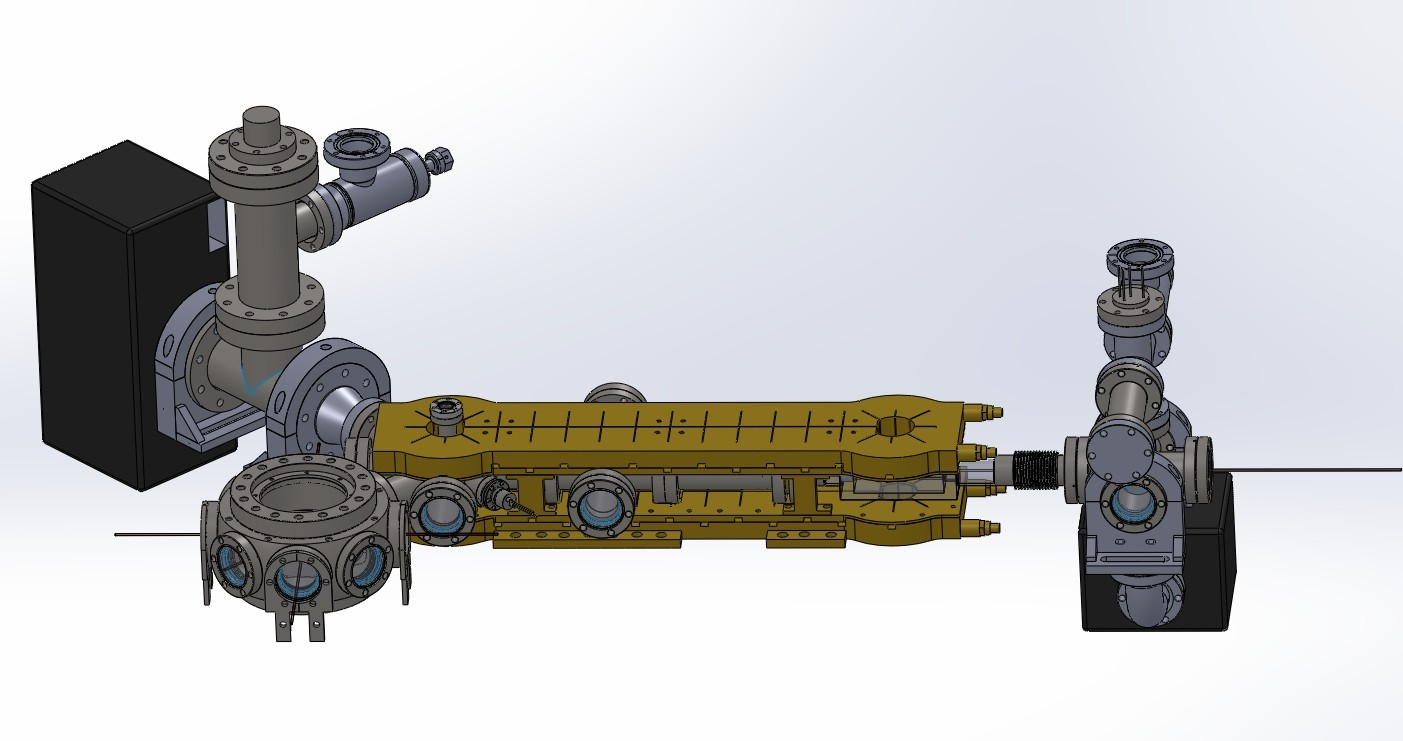
\includegraphics[width=0.7\textwidth]{pict03-01}(注:height=2in也可)
\caption{光晶格实验平台}
\label{fig:pict03-01}
\end{figure}
\end{verbatim}

\begin{figure}[htbp]
\centering
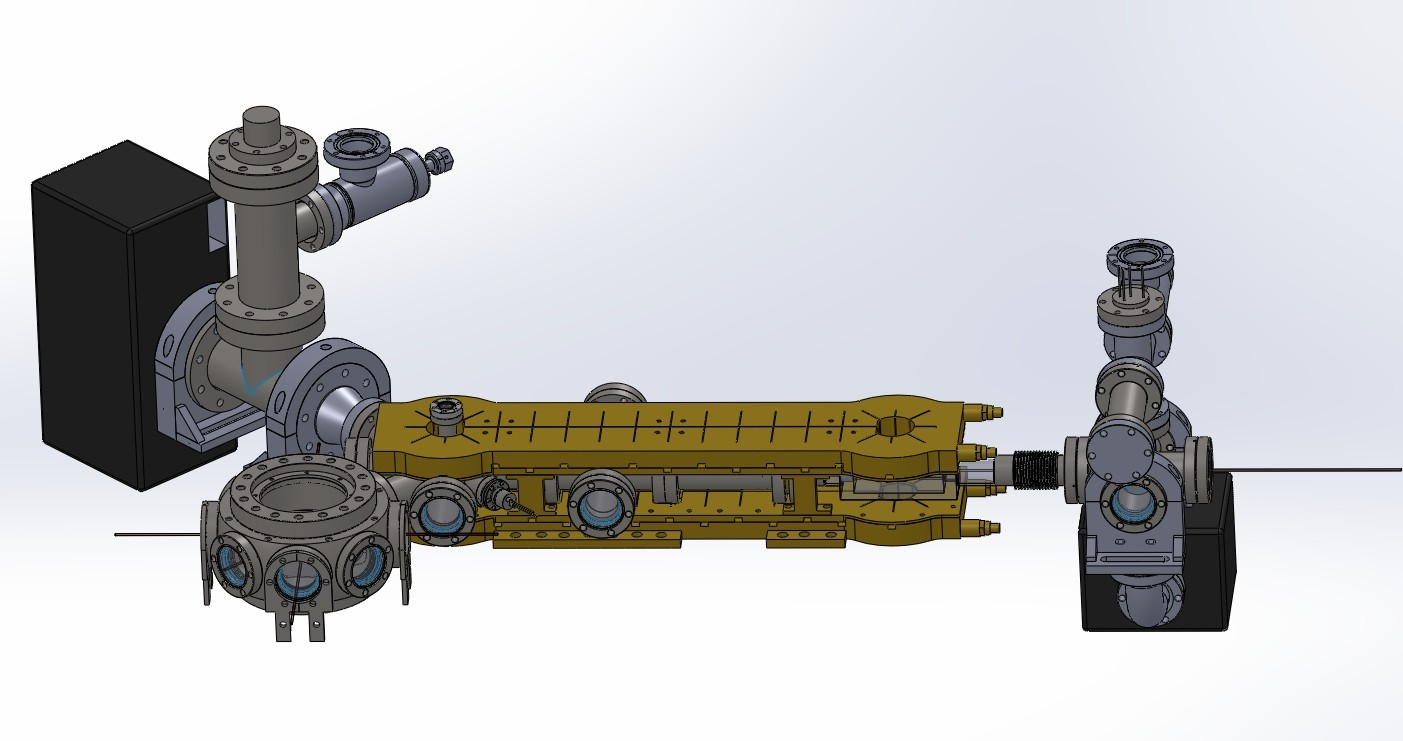
\includegraphics[width=0.7\textwidth]{pict03-01}
\caption{光晶格实验平台}
\label{fig:pict03-01}
\end{figure}

3.双(多)栏插图命令示例:

单标题形式

\begin{verbatim}
\begin{figure}[htbp]
\centering
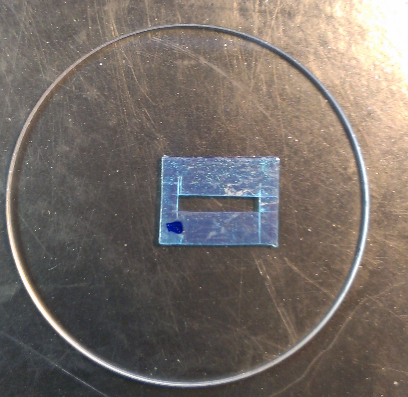
\includegraphics[height=2in]{pict03-04-01}%
\hspace{0.4in}%   (表示两张图片的中间间距,其中的%不可缺失)
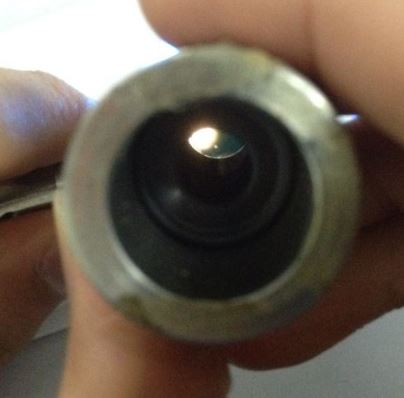
\includegraphics[height=2in]{pict03-04-02}
\figcaption{相位片的示意图}
\label{fig:pict03-04}
\end{figure}
\end{verbatim}

\begin{figure}[htbp]
\centering
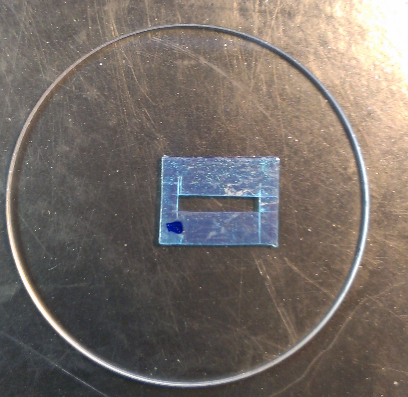
\includegraphics[height=2in]{pict03-04-01}%
\hspace{0.4in}%   
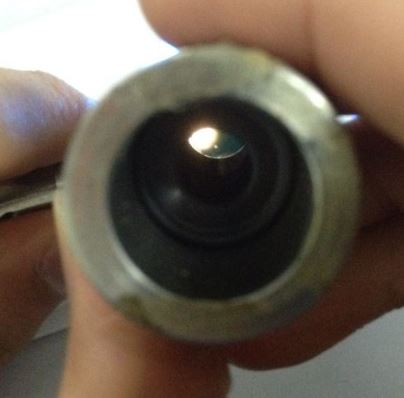
\includegraphics[height=2in]{pict03-04-02}
\caption{相位片的示意图}
\label{fig:pict03-04}
\end{figure}


多标题形式
\begin{verbatim}
\begin{figure}[htbp]
\begin{minipage}[t]{0.5\linewidth}
\centering
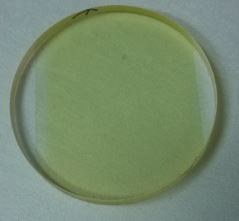
\includegraphics[height=1.6in]{pict04-01}
\caption{ITO镀膜片示意}
\label{fig:pict04-01}
\end{minipage}%
\begin{minipage}[t]{0.5\linewidth}
\centering
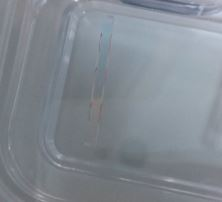
\includegraphics[height=1.6in]{pict04-02}
\caption{二氧化硅镀膜片示意}
\label{fig:pict04-02}
\end{minipage}
\end{figure}
\end{verbatim}

\begin{figure}[htbp]
\begin{minipage}[t]{0.5\linewidth}
\centering
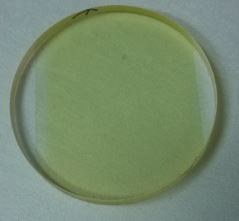
\includegraphics[height=1.8in]{pict04-01}
\caption{ITO镀膜片示意}
\label{fig:pict04-01}
\end{minipage}%
\begin{minipage}[t]{0.5\linewidth}
\centering
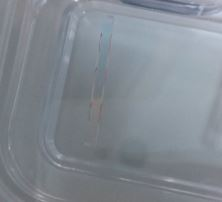
\includegraphics[height=1.8in]{pict04-02}
\caption{二氧化硅镀膜片示意}
\label{fig:pict04-02}
\end{minipage}
\end{figure}

\subsection{表格编辑命令}
一个示例:
\begin{verbatim}
\begin{table}[htbp]
\centering
\caption{通过未镀膜区域的干涉条纹的拟合结果}
\label{tab:chap04-01}
\begin{tabular}{c|c|c|c|c|c}
\hline
拟合函数 & \multicolumn{5}{c}{$y=ae^{-\left(\frac{x-b}{c}\right)^2} \sin(kx+e)$}\\
\hline
拟合参数 & $a$ & $b$ & $c$ & $d$ & $e$\\
\hline
拟合值 & 0.409 & 493.448 & 56.186 & 0.528 & 0.292\\
\hline
\end{tabular}
\end{table}
\end{verbatim}

\begin{table}[htbp]
\centering
\caption{通过未镀膜区域的干涉条纹的拟合结果}
\label{tab:chap04-01}
\begin{tabular}{c|c|c|c|c|c}
\hline
拟合函数 & \multicolumn{5}{c}{$y=ae^{-\left(\frac{x-b}{c}\right)^2} \sin(kx+e)$}\\
\hline
拟合参数 & $a$ & $b$ & $c$ & $d$ & $e$\\
\hline
拟合值 & 0.409 & 493.448 & 56.186 & 0.528 & 0.292\\
\hline
\end{tabular}
\end{table}


%\section{参考文献}
%%%%%%%%%%%%%%%%%%%%%%%%%%%%%%%%%%%%%%%%%%%%%%%%%%%%%%%%%%%%%%%%
%  参考文献
%%%%%%%%%%%%%%%%%%%%%%%%%%%%%%%%%%%%%%%%%%%%%%%%%%%%%%%%%%%%%%%%
\small
\begin{thebibliography}{99}
\setlength{\itemsep}{0pt}
\setlength{\parskip}{0pt}  %段落之间的竖直距离
\bibitem{mc1} Clarke E, Emerson E. Design and synthesis of synchronization skeletons using branching time temporal logic[J]. Logics of Programs, 1982: 52-71.

\bibitem{mc2} Queille J, Sifakis J. Specification and verification of concurrent systems in CESAR[C]//International Symposium on Programming. 1982: 337-351.

\bibitem{mc3}G.O. Clarke, E.M.Emerson. Model Checking[M]. Cambridge: MIT Press, 1999.

\bibitem{np1} Ben-David S. Applications of Description Logic and Causality in Model Checking[D]. University of Waterloo, 2009.

\bibitem{np2} Beer I, Ben-David S, Chockler H, et al. Explaining counterexamples using causality[C]//Computer Aided Verification. 2009: 94-108.

\bibitem{np3} Jalbert N, Sen K. A trace simplification technique for effective debugging of concurrent programs[C]//Proceedings of the eighteenth ACM SIGSOFT international symposium on Foundations of software engineering. 2010: 57-66.
\end{thebibliography}




\newpage  %另起新的一页的命令
%%%%%%%%%%%%%%%%%%%%%%%%%%%%%%%%%%%%%%%%%%%%%%%%%%%%%%%%%%%%%%%%
%  附录
%%%%%%%%%%%%%%%%%%%%%%%%%%%%%%%%%%%%%%%%%%%%%%%%%%%%%%%%%%%%%%%%
\begin{appendix}
\renewcommand{\thesection}{附录~\Alph{section}:}   %格式重命名
\section{计算磁场大小的Mathematica代码}


%完整的文档(程序代码等)引用命令
\begin{verbatim}    

(*-------- Initialization Part --------*)
Clear["Global`*"]
n = 2000;(*times of the lattice depth to recoil Energy*)
t = 10;(*a important fit parameter*)
lambda = 1064*10^-9;(*nm, wave length of laser for optical lattice*)
m = 1.44316*10^-25;(*kg, mass of Rb87*)
muB = 9.274*10^-24;(*J/T, Bohr Magneton*)
hbar = 1.05457*10^-34;(*J*s, Planck's Constant*)
kB = 1.38065*10^-23;(*J/K, Boltzmann's Constant*)

\end{verbatim}

\section{计算能带结构的Mathematica代码(戴汉宁师兄提供)}
\begin{verbatim}

\end{verbatim}
\end{appendix}

\end{document}

